\documentclass[a4paper,12pt]{article}
\usepackage[a4paper, margin=2.5cm]{geometry}
\usepackage[pdftex]{graphicx}
\usepackage{tikz}
\usepackage{pgfplots}
\usepackage{enumitem}
\usepackage{float}
\usepackage[document]{ragged2e}
\usepackage[utf8]{inputenc}
\usepackage[T1]{fontenc}
\usepackage[spanish,es-tabla]{babel}
\renewcommand{\shorthandsspanish}{}
\usepackage{xurl}
\usepackage{lipsum}
\usepackage{mwe}
\usepackage{multirow}
\usepackage{multicol}
\usepackage{siunitx}
\usepackage{listings}
\usepackage{circuitikz}
\usepackage{tabularray}
\usepackage{amsmath}
\usepackage{gensymb}


\usetikzlibrary{arrows.meta,bending}
\graphicspath{ {/home/saikkopat/Documents/ESCOM/FDD/P01/IMG/} }

\usepackage[none]{hyphenat}

\begin{document}

\begin{titlepage}
	\begin{tikzpicture}[overlay, remember picture]
		\path (current page.north east) ++(-0.3,-1.8) node[below left] {
\includegraphics[width=0.35\textwidth]{/home/saikkopat/Documents/LOGOS IPN/EscudoESCOM}};
	\end{tikzpicture}
	\begin{tikzpicture}[overlay, remember picture]
		\path (current page.north west) ++(1.5,-1) node[below right] {
\includegraphics[width=0.2\textwidth]{/home/saikkopat/Documents/LOGOS IPN/logo}};
	\end{tikzpicture}
	\begin{center}
		\vspace{-1.5cm}
		{\LARGE Instituto Politécnico Nacional\par}
		\vspace{.5cm}
		{\LARGE Escuela Superior de Cómputo\par}
		\vspace{.5cm}
		{\Large Departamento de\\Ingeniería en Sistemas Computacionales\par}
		\vspace{2cm}
		{\large Unidad de aprendizaje:}\\{\Large Fundamentos de diseño digital\par}
		\vspace{2cm}
		{\scshape\Huge Práctica 1\par}
		{\itshape\Large Compuertas lógicas\par}
		\vfill
		\vspace{.7cm}
		{\Large Equipo 2\par}
		\vspace{.7cm}
		{\Large Grupo: 3CV2\par}
		\vspace{.7cm}
		{\Large Integrantes:\\González Cárdenas Ángel Aquilez\\Hernández Reyes Diego Alberto\par}
		\vspace{1cm}
		{\Large Profesor: Barrón Vera Josué Emanuel\par}
		\vspace{1cm}
		{\large Fecha de realización: 11 de septiembre de 2023\par}
		{\large Fecha de entrega: 18 de septiembre de 2023\par}
		\vfill
	\end{center}
\end{titlepage} 

\newpage

\tableofcontents

\newpage

\usepgfplotslibrary{units}

\section*{Objetivo}

\textbf{Objetivo}: Al terminar la sesión, los integrantes del equipo contarán con la habilidad de manipular las
compuertas lógicas así como comprobar las tablas de verdad de las compuertas básicas con circuitos integrados.\par

Los alumnos utilizarán los siguientes materiales y equipo:
\vspace{-0.4cm}
\begin{multicols}{2}
\textbf{Equipo}\\
\begin{itemize}[nosep]
		\item 10 \texttt{LEDS} de colores
		\item \texttt{Dip switch}
		\item Fuente de Alimentación
		\item Manual de especificaciones \textit{FAST and LS TTL} de MOTOROLA\textregistered
\end{itemize}

\columnbreak

\textbf{Material}\\
\begin{itemize}[nosep]
		\item \textit{Protoboard}
		\item 1 C. I. 74LS00
		\item 1 C. I. 74LS02
		\item 1 C. I. 74LS04
		\item 1 C. I. 74LS08
		\item 1 C. I. 74LS32
		\item 1 C. I. 74LS86
	
\end{itemize}

\end{multicols}

\section{Desarrollo}

\subsection{Compuertas lógicas}
Primero, se comprobaron los valores teoricos de las compuertas logicas energizandolas y modificando los valores de entrada \emph{A} y \emph{B}, resultando la salida \emph{F}.\par

\subsubsection{Compuerta AND, C. I. 74LS08}
\vspace{-0.3cm}
\begin{figure}[ht!]
\begin{multicols}{2}
	\centering

	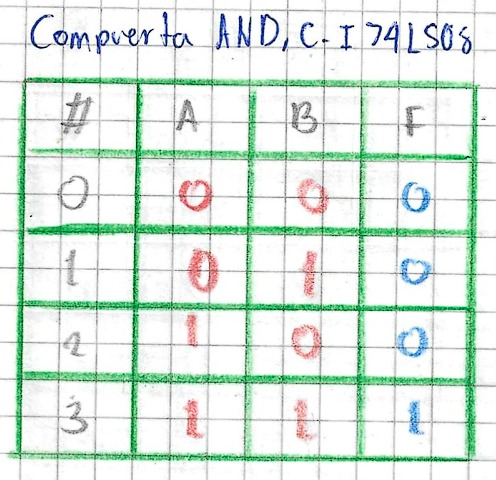
\includegraphics[width=.25\textwidth]{T1}

	\columnbreak
	\begin{minipage}[b]{0.45\linewidth}
	\vspace{1.5cm}
	\centering
	\begin{circuitikz}[american]
		\draw (0,0) node[and port] (and) {};
		\draw (and.in 1) -- ++(-1,0) node[left] {$A$};
    	\draw (and.in 2) -- ++(-1,0) node[left] {$B$};
		\draw (and.out) -- ++(1,0) node[right] {$F$};
	\end{circuitikz}
	\end{minipage}
	
	
\end{multicols}
\vspace{-0.5cm}
	\caption{\textbf{Tabla de verdad y diagrama de la compuerta AND}}
\end{figure}


\begin{figure}[ht!]
\begin{multicols}{2}
	\centering

		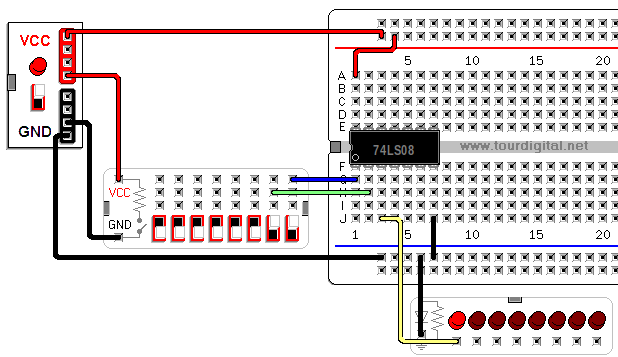
\includegraphics[width=.55\textwidth]{AND}

	\columnbreak

		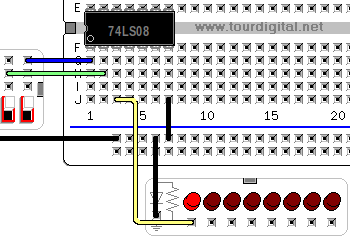
\includegraphics[width=.25\textwidth]{AND1}
		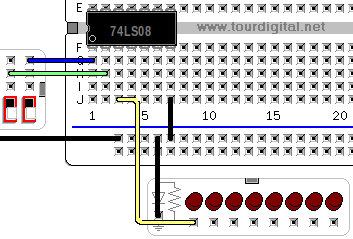
\includegraphics[width=.25\textwidth]{AND2}

\end{multicols}
\vspace{-0.5cm}
\caption{\textbf{Compuerta AND en funcionamiento}}
\end{figure}

\newpage

\subsubsection{Compuerta OR C. I. 74LS32}
\begin{figure}[ht!]
\begin{multicols}{2}
	\centering

	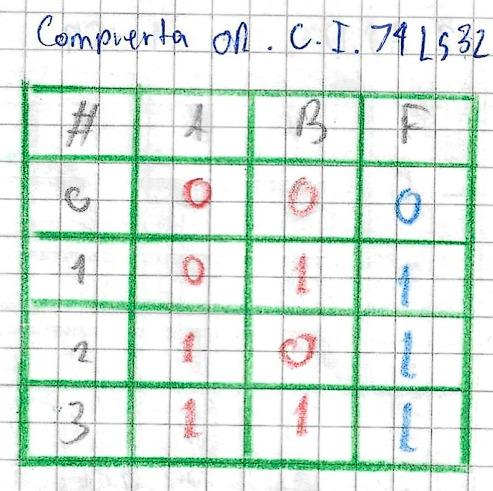
\includegraphics[width=.3\textwidth]{T2}

	\columnbreak
	\begin{minipage}[b]{0.45\linewidth}
	\vspace{1.5cm}
	\centering
	\begin{circuitikz}[american]
		\draw (0,0) node[or port] (or) {};
		\draw (or.in 1) -- ++(-1,0) node[left] {$A$};
    	\draw (or.in 2) -- ++(-1,0) node[left] {$B$};
		\draw (or.out) -- ++(1,0) node[right] {$F$};
	\end{circuitikz}
	\end{minipage}
	
	
\end{multicols}
\vspace{-0.5cm}
	\caption{\textbf{Tabla de verdad y diagrama de la compuerta OR}}
\end{figure}

\begin{figure}[ht!]
\begin{multicols}{2}
	\centering

		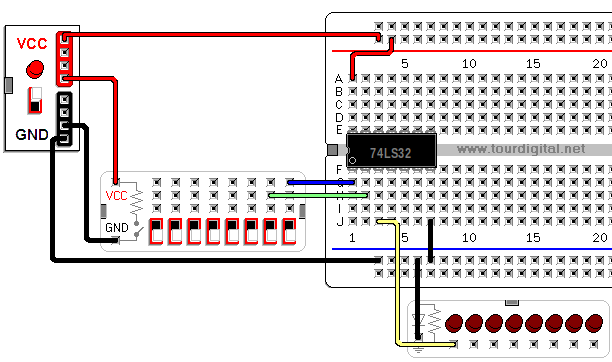
\includegraphics[width=.55\textwidth]{OR}

	\columnbreak

		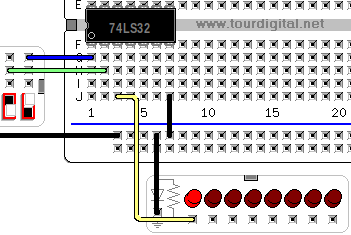
\includegraphics[width=.3\textwidth]{OR1}
		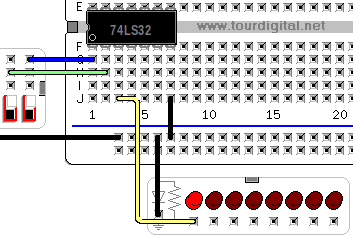
\includegraphics[width=.3\textwidth]{OR2}

\end{multicols}
\vspace{-0.5cm}
\caption{\textbf{Compuerta OR en funcionamiento}}
\end{figure}

\subsubsection{Compuerta NAND C. I. 74LS00}
\begin{figure}[ht!]
\begin{multicols}{2}
	\centering

	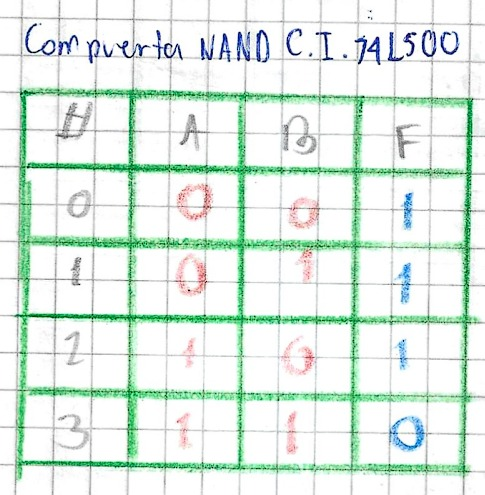
\includegraphics[width=.3\textwidth]{T3}

	\columnbreak
	\begin{minipage}[b]{0.45\linewidth}
	\vspace{1.5cm}
	\centering
	\begin{circuitikz}[american]
		\draw (0,0) node[nand port] (nand) {};
		\draw (nand.in 1) -- ++(-1,0) node[left] {$A$};
    	\draw (nand.in 2) -- ++(-1,0) node[left] {$B$};
		\draw (nand.out) -- ++(1,0) node[right] {$F$};
	\end{circuitikz}
	\end{minipage}
	
\end{multicols}
\vspace{-0.5cm}
	\caption{\textbf{Tabla de verdad y diagrama de la compuerta NAND}}
\end{figure}

\newpage

\begin{figure}[ht!]
\begin{multicols}{2}
	\centering

		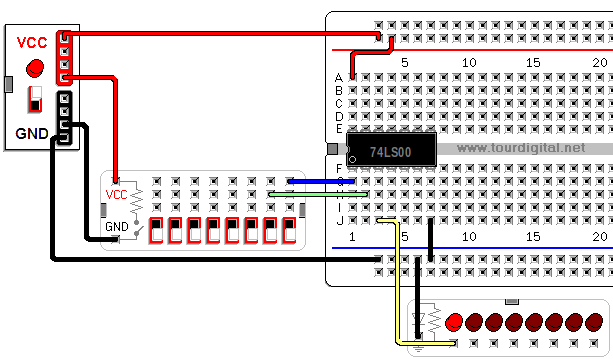
\includegraphics[width=.55\textwidth]{NAND}

	\columnbreak

		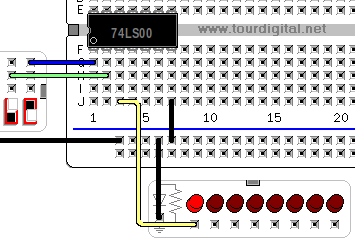
\includegraphics[width=.3\textwidth]{NAND1}
		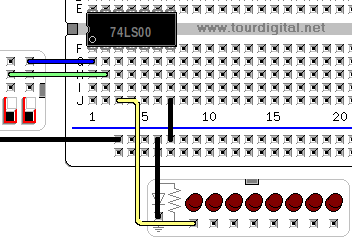
\includegraphics[width=.3\textwidth]{NAND2}

\end{multicols}
\vspace{-0.5cm}
\caption{\textbf{Compuerta NAND en funcionamiento}}
\end{figure}


\subsubsection{Compuerta NOR C. I. 74LS02}

\begin{figure}[ht!]
\begin{multicols}{2}
	\centering

	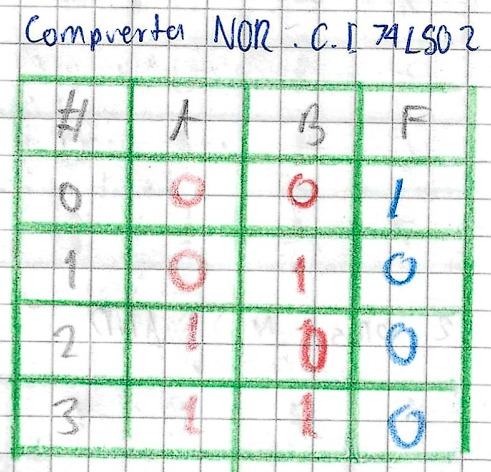
\includegraphics[width=.3\textwidth]{T4}

	\columnbreak
	\begin{minipage}[b]{0.45\linewidth}
	\vspace{1.5cm}
	\centering
	\begin{circuitikz}[american]
		\draw (0,0) node[nor port] (nor) {};
		\draw (nor.in 1) -- ++(-1,0) node[left] {$A$};
    	\draw (nor.in 2) -- ++(-1,0) node[left] {$B$};
		\draw (nor.out) -- ++(1,0) node[right] {$F$};
	\end{circuitikz}
	\end{minipage}
	
	
\end{multicols}
\vspace{-0.5cm}
\caption{\textbf{Tabla de verdad y diagrama de la compuerta NOR}}
\end{figure}

\begin{figure}[ht!]
\begin{multicols}{2}
	\centering

		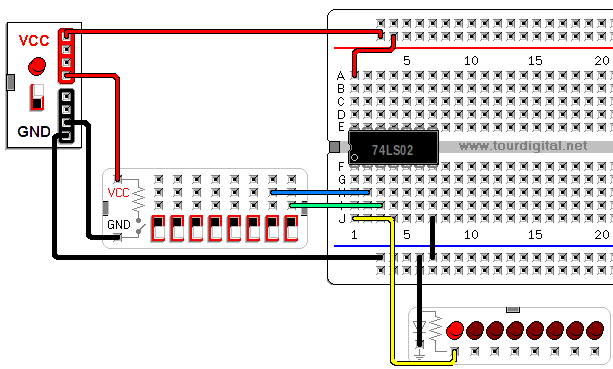
\includegraphics[width=.55\textwidth]{NOR}

	\columnbreak

		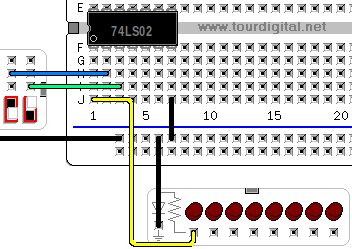
\includegraphics[width=.3\textwidth]{NOR1}
		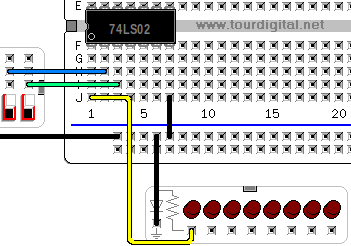
\includegraphics[width=.3\textwidth]{NOR2}

\end{multicols}
\vspace{-0.5cm}
\caption{\textbf{Compuerta NOR en funcionamiento}}
\end{figure}

\newpage


\subsubsection{Compuerta XOR C. I. 74LS86}

\begin{figure}[ht!]
\begin{multicols}{2}
	\centering

	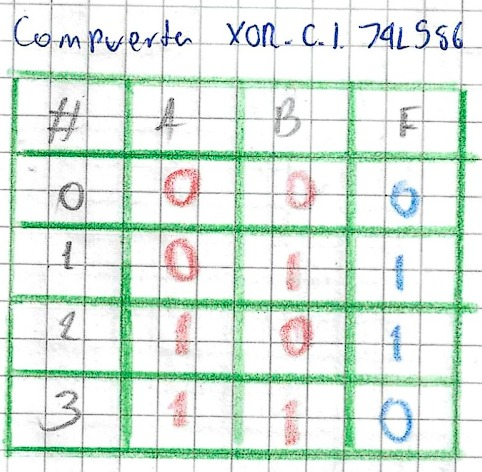
\includegraphics[width=.3\textwidth]{T5}

	\columnbreak
	\begin{minipage}[b]{0.45\linewidth}
	\vspace{1.5cm}
	\centering
	\begin{circuitikz}[american]
		\draw (0,0) node[xor port] (xor) {};
		\draw (xor.in 1) -- ++(-1,0) node[left] {$A$};
    	\draw (xor.in 2) -- ++(-1,0) node[left] {$B$};
		\draw (xor.out) -- ++(1,0) node[right] {$F$};
	\end{circuitikz}
	\end{minipage}
	
	
\end{multicols}
\vspace{-0.5cm}
\caption{\textbf{Tabla de verdad y diagrama de la compuerta XOR}}
\end{figure}

\begin{figure}[ht!]
\begin{multicols}{2}
	\centering

		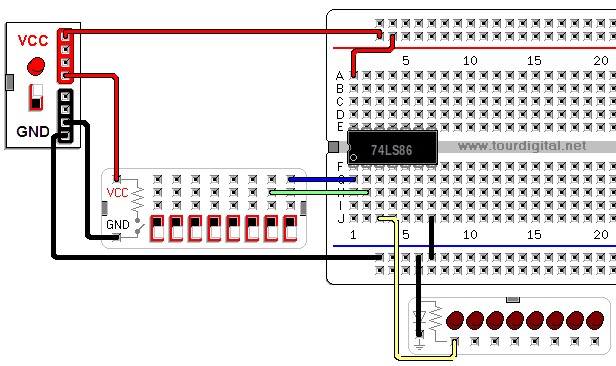
\includegraphics[width=.55\textwidth]{XOR}

	\columnbreak

		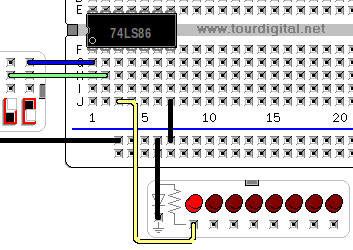
\includegraphics[width=.3\textwidth]{XOR1}
		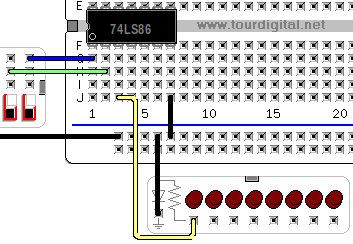
\includegraphics[width=.3\textwidth]{XOR2}

\end{multicols}
\vspace{-0.5cm}
\caption{\textbf{Compuerta XOR en funcionamiento}}
\end{figure}


\subsubsection{Compuerta XNOR C. I. 74LS86 + 74LS04}

\begin{figure}[ht!]
\begin{multicols}{2}
	\centering

	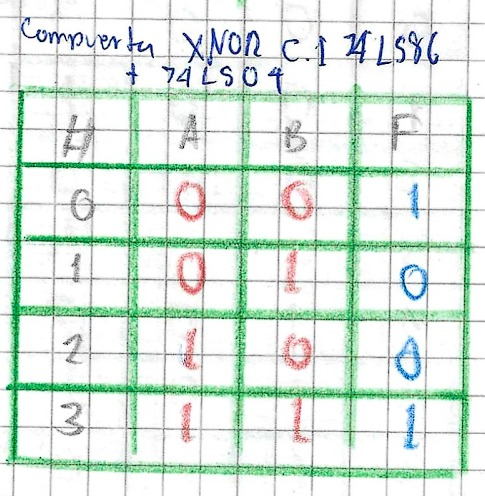
\includegraphics[width=.3\textwidth]{T6}

	\columnbreak
	\begin{minipage}[b]{0.45\linewidth}	
	\vspace{1.5cm}
	\centering
	\begin{circuitikz}[american]
		\draw (0,0) node[xnor port] (xnor) {};
		\draw (xnor.in 1) -- ++(-1,0) node[left] {$A$};
    	\draw (xnor.in 2) -- ++(-1,0) node[left] {$B$};
		\draw (xnor.out) -- ++(1,0) node[right] {$F$};
	\end{circuitikz}
	\end{minipage}
	
	
\end{multicols}
\vspace{-0.5cm}
\caption{\textbf{Tabla de verdad y diagrama de la compuerta XNOR}}
\end{figure}

\newpage

\begin{figure}[ht!]
\begin{multicols}{2}
	\centering

		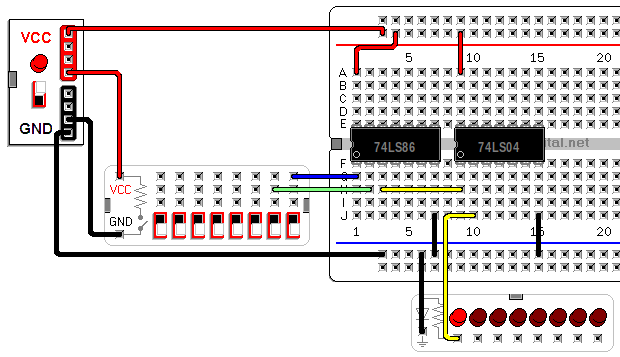
\includegraphics[width=.55\textwidth]{XNOR}

	\columnbreak

		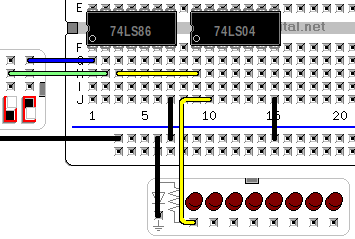
\includegraphics[width=.3\textwidth]{XNOR1}
		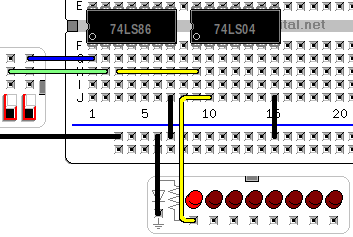
\includegraphics[width=.3\textwidth]{XNOR2}

\end{multicols}
\vspace{-0.5cm}
\caption{\textbf{Compuerta XNOR en funcionamiento}}
\end{figure}


\newpage

\subsection{Circuitos combinacionales}

Arme los siguientes circuitos y verifique sus valores de salida para los diferentes valores de entrada.\par

\subsubsection{Circuito 1}

\begin{figure}[ht!]
\begin{multicols}{2}
	\centering

	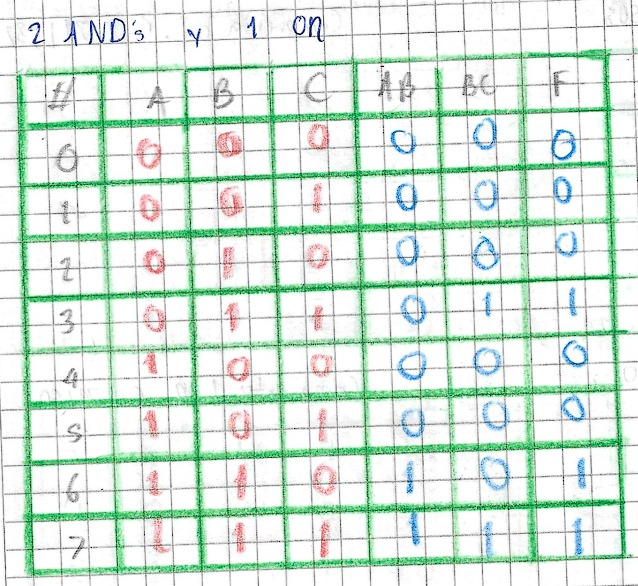
\includegraphics[width=.3\textwidth]{T7}

	\columnbreak
	\begin{minipage}[b]{0.45\linewidth}
	\vspace{.5cm}
	\centering
	\begin{circuitikz}[american]
		\draw (0,2) node[and port] (or1) {}
		(0,0) node[and port] (or2) {}
		(2,1) node[or port] (and) {}
		(or1.out) -| (and.in 1)
		(or2.out) -| (and.in 2);
		\draw (or1.in 1) -- ++(-1,0) node[left] {$A$};
		\draw (or1.in 2) -- ++(-1,0) node[left] {$B$};
		\draw (or2.in 1) -- ++(-1,0) node[left] {$B$};
    	\draw (or2.in 2) -- ++(-1,0) node[left] {$C$};
		\draw (and.out) -- ++(.5,0) node[right] {$F$};
	\end{circuitikz}
	\end{minipage}
	
	
\end{multicols}
\vspace{-0.5cm}
\caption{\textbf{Tabla de verdad y diagrama del Circuito 1}}
\end{figure}

\begin{figure}[ht!]
\centering
	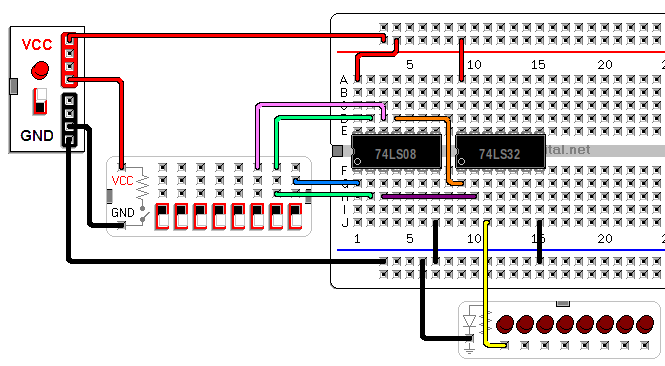
\includegraphics[width=.6\textwidth]{A}
\end{figure}

\begin{figure}[ht!]
\begin{multicols}{2}
	\centering

		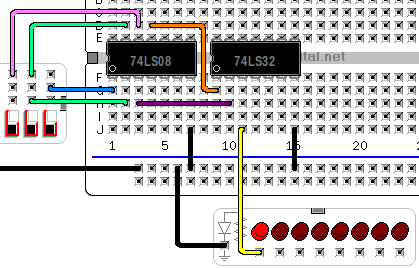
\includegraphics[width=.35\textwidth]{A1}
		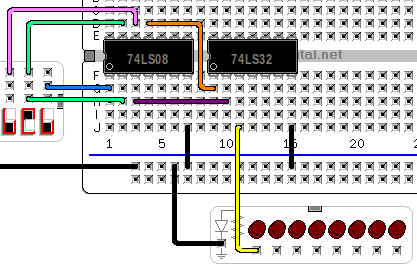
\includegraphics[width=.35\textwidth]{A2}

	\columnbreak

		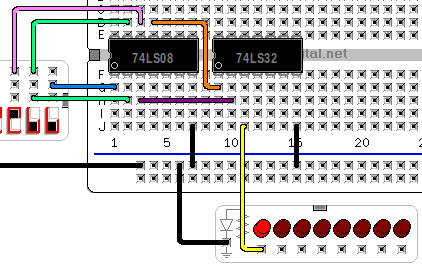
\includegraphics[width=.35\textwidth]{A3}
		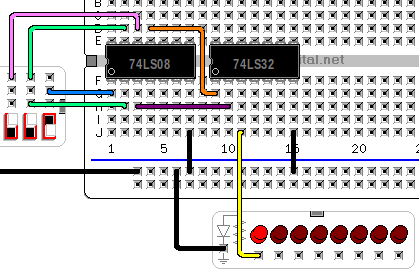
\includegraphics[width=.35\textwidth]{A4}

\end{multicols}
\vspace{-0.5cm}
\caption{\textbf{Circuito 1 en funcionamiento}}
\end{figure}


\newpage

\subsubsection{Circuito 2}

\begin{figure}[ht!]
\begin{multicols}{2}
	\centering

	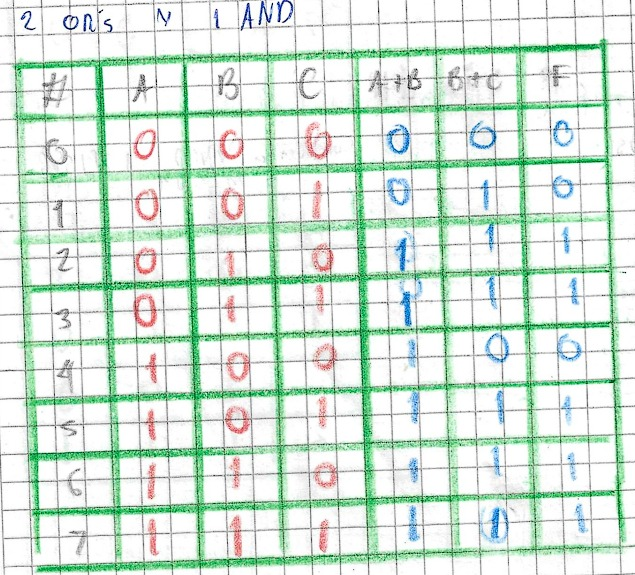
\includegraphics[width=.3\textwidth]{T8}

	\columnbreak
	\begin{minipage}[b]{0.45\linewidth}
	\vspace{.5cm}
	\centering
	\begin{circuitikz}[american]
		\draw (0,2) node[or port] (or1) {}
		(0,0) node[or port] (or2) {}
		(2,1) node[and port] (and) {}
		(or1.out) -| (and.in 1)
		(or2.out) -| (and.in 2);
		\draw (or1.in 1) -- ++(-1,0) node[left] {$A$};
		\draw (or1.in 2) -- ++(-1,0) node[left] {$B$};
		\draw (or2.in 1) -- ++(-1,0) node[left] {$B$};
    	\draw (or2.in 2) -- ++(-1,0) node[left] {$C$};
		\draw (and.out) -- ++(.5,0) node[right] {$F$};
	\end{circuitikz}
	\end{minipage}
	
	
\end{multicols}
\vspace{-0.5cm}
\caption{\textbf{Tabla de verdad y diagrama del Circuito 2}}
\end{figure}

\begin{figure}[ht!]
\centering
	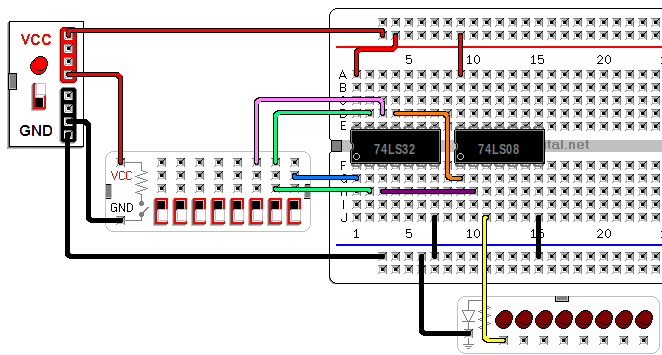
\includegraphics[width=.7\textwidth]{B}
\end{figure}

\begin{figure}[ht!]
\begin{multicols}{2}
	\centering

		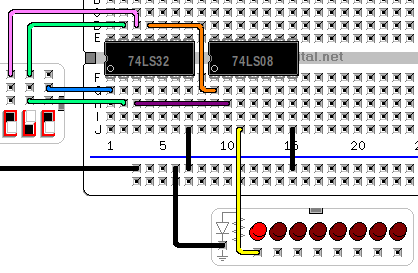
\includegraphics[width=.4\textwidth]{B1}
		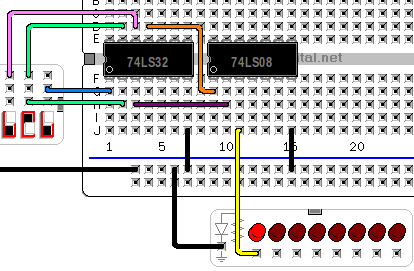
\includegraphics[width=.4\textwidth]{B2}

	\columnbreak

		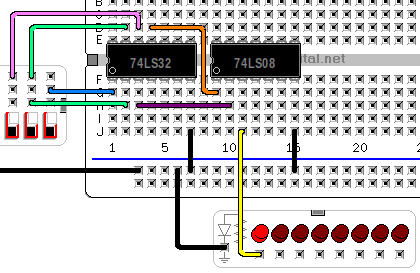
\includegraphics[width=.4\textwidth]{B3}
		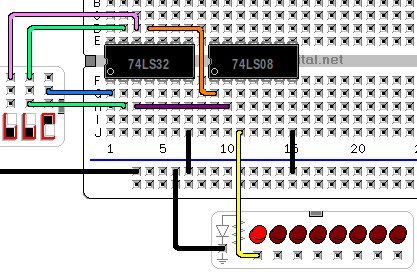
\includegraphics[width=.4\textwidth]{B4}

\end{multicols}
\vspace{-0.5cm}
\caption{\textbf{Circuito 2 en funcionamiento}}
\end{figure}

\newpage

\subsubsection{Circuito 3}

\begin{figure}[ht!]
\begin{multicols}{2}
	\centering

	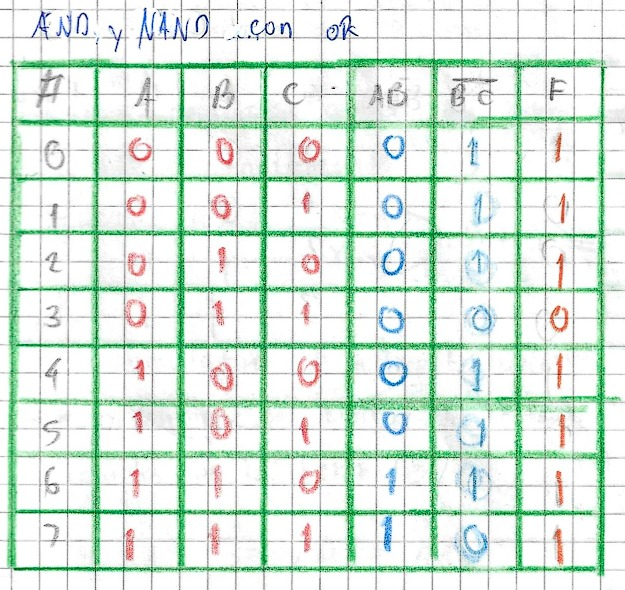
\includegraphics[width=.3\textwidth]{T9}

	\columnbreak
	\begin{minipage}[b]{0.45\linewidth}
	\vspace{.5cm}
	\centering
	\begin{circuitikz}[american]
		\draw (0,2) node[and port] (or1) {}
		(0,0) node[nand port] (or2) {}
		(2,1) node[or port] (and) {}
		(or1.out) -| (and.in 1)
		(or2.out) -| (and.in 2);
		\draw (or1.in 1) -- ++(-1,0) node[left] {$A$};
		\draw (or1.in 2) -- ++(-1,0) node[left] {$B$};
		\draw (or2.in 1) -- ++(-1,0) node[left] {$B$};
    	\draw (or2.in 2) -- ++(-1,0) node[left] {$C$};
		\draw (and.out) -- ++(.5,0) node[right] {$F$};
	\end{circuitikz}
	\end{minipage}
	
	
\end{multicols}
\vspace{-0.5cm}
\caption{\textbf{Tabla de verdad y diagrama del Circuito 3}}
\end{figure}

\begin{figure}[ht!]
\centering
	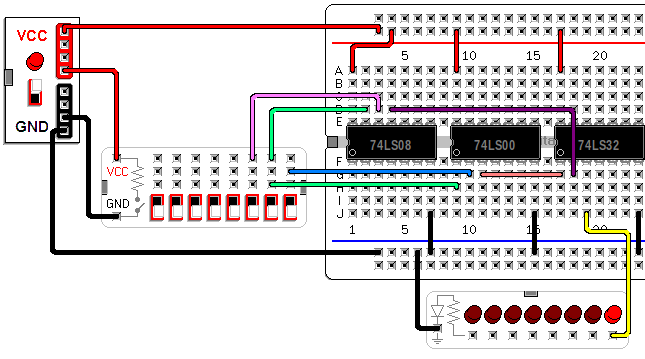
\includegraphics[width=.7\textwidth]{C}
\end{figure}

\begin{figure}[ht!]
\begin{multicols}{2}
	\centering

		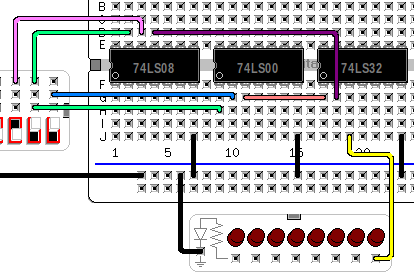
\includegraphics[width=.4\textwidth]{C1}
		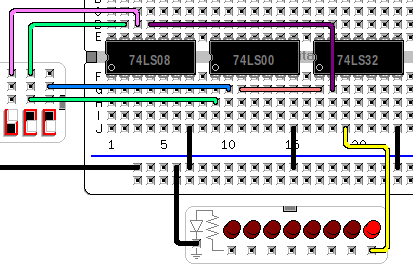
\includegraphics[width=.4\textwidth]{C2}

	\columnbreak

		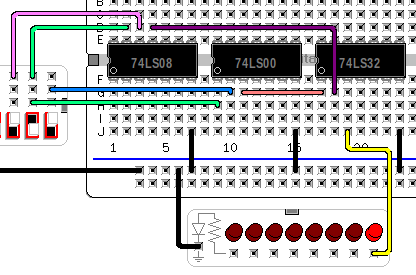
\includegraphics[width=.4\textwidth]{C3}
		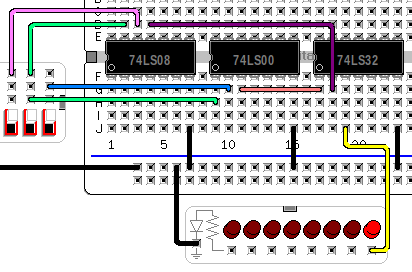
\includegraphics[width=.4\textwidth]{C4}

\end{multicols}
\vspace{-0.5cm}
\caption{\textbf{Circuito 3 en funcionamiento}}
\end{figure}


\newpage

\subsubsection{Circuito 4}

\begin{figure}[ht!]
\begin{multicols}{2}
	\centering

	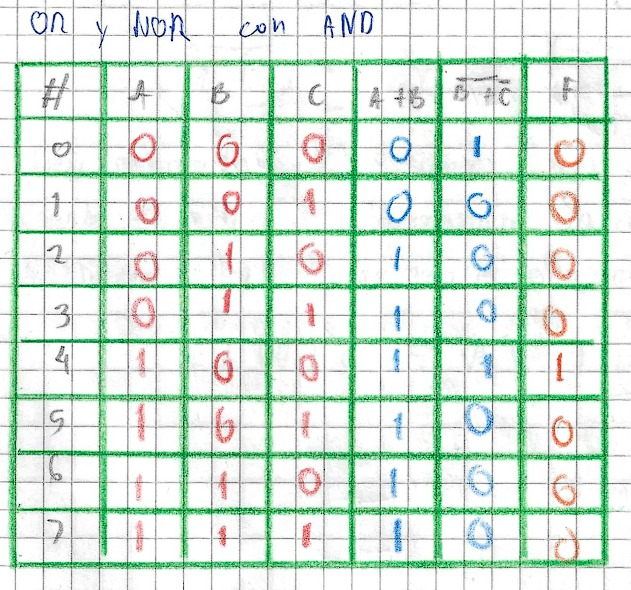
\includegraphics[width=.3\textwidth]{T10}

	\columnbreak
	\begin{minipage}[b]{0.45\linewidth}
	\vspace{.5cm}
	\centering
	\begin{circuitikz}[american]
		\draw (0,2) node[or port] (or1) {}
		(0,0) node[nor port] (or2) {}
		(2,1) node[and port] (and) {}
		(or1.out) -| (and.in 1)
		(or2.out) -| (and.in 2);
		\draw (or1.in 1) -- ++(-1,0) node[left] {$A$};
		\draw (or1.in 2) -- ++(-1,0) node[left] {$B$};
		\draw (or2.in 1) -- ++(-1,0) node[left] {$B$};
    	\draw (or2.in 2) -- ++(-1,0) node[left] {$C$};
		\draw (and.out) -- ++(.5,0) node[right] {$F$};
	\end{circuitikz}
	\end{minipage}
	
	
\end{multicols}
\vspace{-0.5cm}
\caption{\textbf{Tabla de verdad y diagrama del Circuito 4}}
\end{figure}

\begin{figure}[ht!]
\centering
	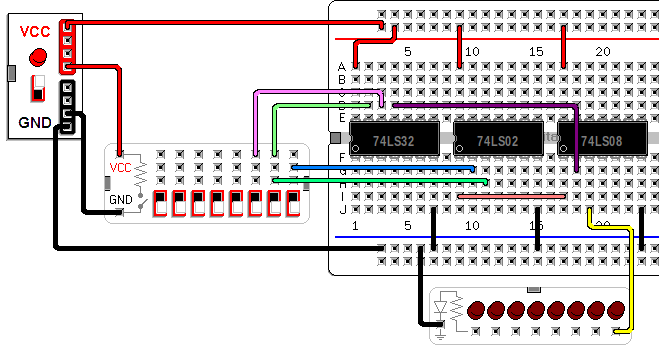
\includegraphics[width=.7\textwidth]{D}
\end{figure}

\begin{figure}[ht!]
\begin{multicols}{2}
	\centering

		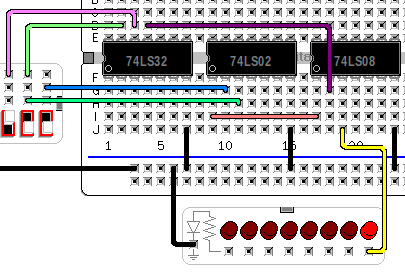
\includegraphics[width=.4\textwidth]{D1}
		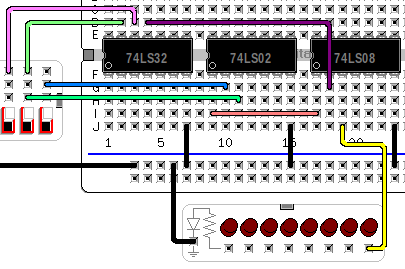
\includegraphics[width=.4\textwidth]{D2}

	\columnbreak

		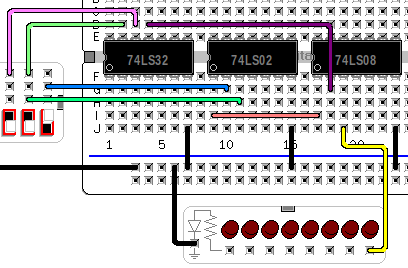
\includegraphics[width=.4\textwidth]{D3}
		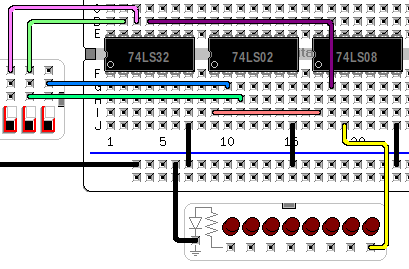
\includegraphics[width=.4\textwidth]{D4}

\end{multicols}
\vspace{-0.5cm}
\caption{\textbf{Circuito 4 en funcionamiento}}
\end{figure}

\newpage

\subsubsection{Circuito 5}

\begin{figure}[ht!]
\begin{multicols}{2}
	\centering

	\includegraphics[width=.4\textwidth]{T11}

	\columnbreak
	
	\includegraphics[width=.5\textwidth]{DIG5}
	
\end{multicols}
\vspace{-0.5cm}
\caption{\textbf{Tabla de verdad y diagrama del Circuito 5}}
\end{figure}

\begin{figure}[ht!]
\centering
	\includegraphics[width=.7\textwidth]{E}
\end{figure}

\begin{figure}[ht!]
\begin{multicols}{2}
	\centering

		\includegraphics[width=.4\textwidth]{E1}

	\columnbreak

		\includegraphics[width=.4\textwidth]{E2}

\end{multicols}
\vspace{-0.5cm}
\caption{\textbf{Circuito 5 en funcionamiento}}
\end{figure}

\newpage

\subsubsection{Circuito 6}

\begin{figure}[ht!]
\begin{multicols}{2}
	\centering

	\includegraphics[width=.4\textwidth]{T12}

	\columnbreak
	
	\includegraphics[width=.5\textwidth]{DIG6}
	
\end{multicols}
\vspace{-0.5cm}
\caption{\textbf{Tabla de verdad y diagrama del Circuito 6}}
\end{figure}

\begin{figure}[ht!]
\centering
	\includegraphics[width=.7\textwidth]{F}
\end{figure}

\begin{figure}[ht!]
\begin{multicols}{2}
	\centering

		\includegraphics[width=.4\textwidth]{F1}

	\columnbreak

		\includegraphics[width=.4\textwidth]{F2}

\end{multicols}
\vspace{-0.5cm}
\caption{\textbf{Circuito 6 en funcionamiento}}
\end{figure}


\newpage

\section{Observaciones y conclusiones}

González Cárdenas Ángel Aquilez

\begin{quotation}
	Al finalizar el desarrollo de la práctica, se adquirió la capacidad de armar correctamente circuitos utilizando compuertas lógicas, así como se demostró una comprensión sólida de la lógica binaria y cómo se pueden utilizar para realizar operaciones específicas.
	Cabe destacar la implementación de una puerta XNOR a partir de una XOR y una NOT debido a la limitante del simulador de un componente de tales características, y como se consiguió un circuito equivalente.\par

	Este conocimiento es esencial en numerosas aplicaciones de la electrónica y la informática.\par

	Además, cabe destacar la necesidad de la precisión durante el armado de un circuito, ya que un simple error de conexión o una comprensión incorrecta de cómo funcionan las compuertas lógicas pueden llevar a resultados incorrectos en la salida del circuito.\par
\end{quotation}

\vspace{1cm}

Hernández Reyes Diego Alberto

\begin{quotation}
	Al finalizar la sesión, se adquirió la habilidad de manipular las compuertas lógicas y la verificación de las tablas de verdad de las compuertas básicas mediante circuitos integrados. También se reafirmaron los conocimientos de operaciones de números binarios.\par

	La habilidad para manipular compuertas lógicas es esencial en numerosas aplicaciones, desde la construcción de circuitos electrónicos simples hasta el diseño y la programación de sistemas más complejos.\par

	La verificación de las tablas de verdad de las compuertas básicas utilizando circuitos integrados es una excelente manera de consolidar este conocimiento. Permite a los miembros del equipo comprobar de manera Esta experiencia práctica es crucial para la comprensión profunda de los principios de la electrónica digital y la lógica booleana. \par
\end{quotation}

\end{document}